\section{Projekt mit CMake}

\begin{frame}[fragile]
    \frametitle{CMakeLists.txt Datei}


    \begin{minted}{bash}
cmake_minimum_required(VERSION 3.15)
project(openmp_emboss)
set(CMAKE_CXX_STANDARD 17)
file(COPY "resources/images" DESTINATION "resources")

find_package(OpenMP REQUIRED)
find_package(OpenCV REQUIRED)

add_executable(openmp_emboss main.cpp)
target_link_libraries(
        openmp_emboss
        PUBLIC OpenMP::OpenMP_CXX
        ${OpenCV_LIBS}
)        
    \end{minted}
\end{frame}

\section {Allgemeines}

\begin{frame}
    \frametitle{Allgemeines}

    \begin{itemize}
        \item Alle Algorithmen bestehen aus 2 geschachtelten For-Schleifen, die über alle Pixel iterieren
        \item Drei Varianten pro Algorithmus: Äußere Schleife, Innere Schleife, Collapse(2)
        \item Zeitmessungen mit 1-16 Threads durchgeführt
        \item Arithmetisches Mittel über 20 Iterationen
    \end{itemize}
\end{frame}


\section{Grayscale}

\begin{frame}
    \frametitle{Grayscale}

    \begin{itemize}
        \item Wandelt drei Farbwerte in einen Schwarz-Weis-Wert um \pause
        \item Zwei verschiedene Formeln \pause
        \item OpenCV\footnote{OpenCV wurde in der Implementierung verwendet}: $ f(r, g, b) = 0.21r + 0.72g + 0.07b $  \pause
        \item Luminosity: $ f(r, g, b) =  0.299r + 0.587g + 0.114b $ \pause
    \end{itemize}
\end{frame}

\begin{frame}
    \frametitle{Grayscale - Ergebnisse}

    \begin{figure}[H]
        \centering
    
        \includegraphics[width=0.30\textwidth]{images/dice.png}
        \includegraphics[width=0.30\textwidth]{images/cv-grayscale.png}
        \includegraphics[width=0.30\textwidth]{images/own-grayscale.png}
        
        \begin{center}
            \caption{Grayscale results of OpenCV (middle) and self-implemented  Algorithm (right)}            
        \end{center}

        \label{fig:grayscale}
    \end{figure}
\end{frame}


\begin{frame}
    \frametitle{Grayscale - Performance}

    \begin{center}
        \begin{figure}[H]
            \centering
    
            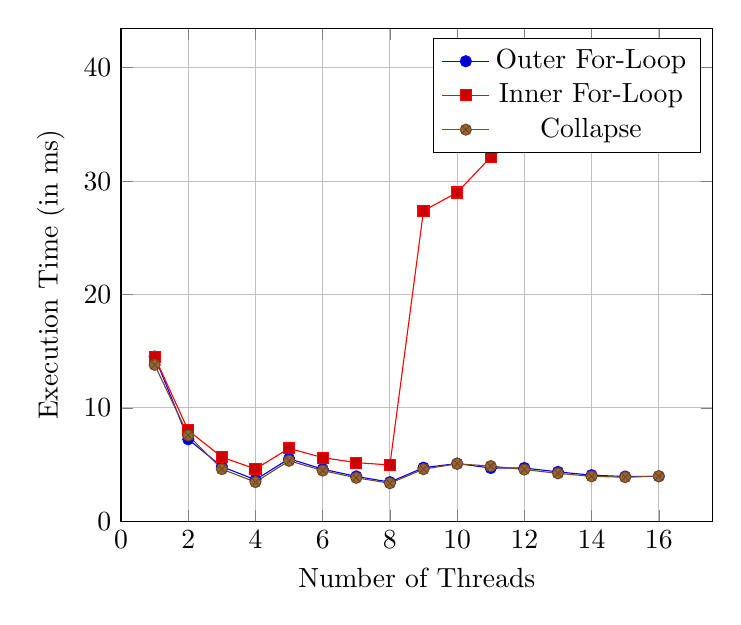
\begin{tikzpicture}
                \begin{axis}[
                    title={},
                    width=0.75\textwidth,
                    xlabel={Number of Threads},
                    ylabel={Execution Time (in ms)},
                    xmin=0,
                    ymin=0,
                    grid=major
                ]
                    \addplot coordinates {
                        (1,14.529)(2,7.2352)(3,4.82325)(4,3.66465)(5,5.51725)(6,4.6023)(7,3.9593)(8,3.4559)(9,4.73325)(10,5.0951)(11,4.7007)(12,4.70275)(13,4.3584)(14,4.0717)(15,3.9503)(16,3.96975)
                    };
                    \addlegendentry{Outer For-Loop}
    
                    \addplot coordinates {
                        (1,14.5167)(2,8.0113)(3,5.6654)(4,4.6173)(5,6.4365)(6,5.61665)(7,5.17615)(8,4.9681)(9,27.3852)(10,28.9996)(11,32.1199)(12,33.9853)(13,34.6872)(14,36.0339)(15,38.6033)(16,39.5345)
                    };
                    \addlegendentry{Inner For-Loop}       
    
                    \addplot coordinates {
                        (1,13.802)(2,7.58295)(3,4.6058)(4,3.4596)(5,5.33955)(6,4.4732)(7,3.8374)(8,3.359)(9,4.60065)(10,5.069)(11,4.8751)(12,4.56545)(13,4.22825)(14,3.9661)(15,3.8909)(16,3.98015)
                    };
                    \addlegendentry{Collapse}
                \end{axis}
            \end{tikzpicture}
            \caption{Grayscale Performance Tests}
        \end{figure}
    \end{center}
\end{frame}



\begin{frame}
    \frametitle{HSV - Ergebnisse}

    
    \begin{figure}[H]
        \centering
    
        \includegraphics[width=0.30\textwidth]{images/dice.png}
        \includegraphics[width=0.30\textwidth]{images/cv-hsv.png}
        \includegraphics[width=0.30\textwidth]{images/own-hsv.png}
        
        \caption{RGB to HSV results of OpenCV (middle) and self-implemented  Algorithm (right)}
        \label{fig:hsv}
    \end{figure}
\end{frame}


\begin{frame}
    \frametitle{HSV - Performance}

    \begin{center}
        \begin{figure}[H]
            \centering
    
            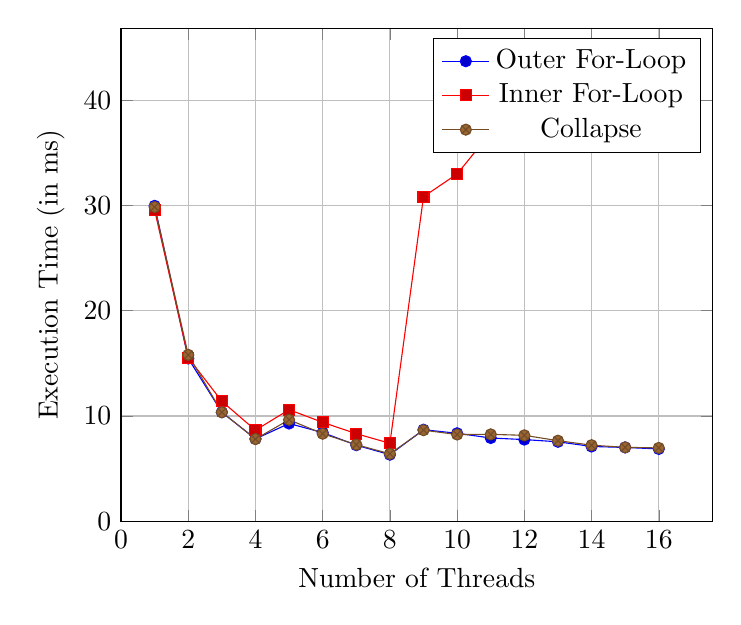
\begin{tikzpicture}
                \begin{axis}[
                    title={},
                    width=0.75\textwidth,
                    xlabel={Number of Threads},
                    ylabel={Execution Time (in ms)},
                    xmin=0,
                    ymin=0,
                    grid=major
                ]
                    \addplot coordinates {
                        (1,29.9648)(2,15.469)(3,10.3609)(4,7.82855)(5,9.2882)(6,8.43245)(7,7.2304)(8,6.32945)(9,8.70195)(10,8.3631)(11,7.9136)(12,7.7625)(13,7.5532)(14,7.10865)(15,7.01605)(16,6.8747)
                    };
                    \addlegendentry{Outer For-Loop}
    
                    \addplot coordinates {
                        (1,29.5613)(2,15.5333)(3,11.4017)(4,8.653)(5,10.6025)(6,9.40055)(7,8.3203)(8,7.4095)(9,30.8314)(10,32.9906)(11,36.9195)(12,36.351)(13,37.3633)(14,39.1266)(15,41.8026)(16,42.5773)
                    };
                    \addlegendentry{Inner For-Loop}
                    
                    \addplot coordinates {
                        (1,29.848)(2,15.812)(3,10.3598)(4,7.8134)(5,9.64615)(6,8.31875)(7,7.27835)(8,6.4122)(9,8.6546)(10,8.2441)(11,8.26075)(12,8.16765)(13,7.66035)(14,7.2298)(15,7.02725)(16,6.97055)

                    };
                    \addlegendentry{Collapse}   
                \end{axis}
            \end{tikzpicture}
            \caption{RGB to HSV Performance Tests}
        \end{figure}
    \end{center}    
\end{frame}

\section{Emboss}

\begin{frame}
    \frametitle{Emboss}

    \begin{itemize}
        \item 
    \end{itemize}
\end{frame}

\begin{frame}
    \frametitle{Emboss - Ergebnisse}

    \begin{figure}[H]
        \centering
    
        \includegraphics[width=0.30\textwidth]{images/dice.png}
        \includegraphics[width=0.30\textwidth]{images/own-emboss.png}
        
        \caption{Results of self-implemented Emboss-Algorithm}
        \label{fig:emboss}
    \end{figure}
\end{frame}


\begin{frame}
    \frametitle{Emboss - Performance}

    \begin{center}
        \begin{figure}[H]
            \centering
            
            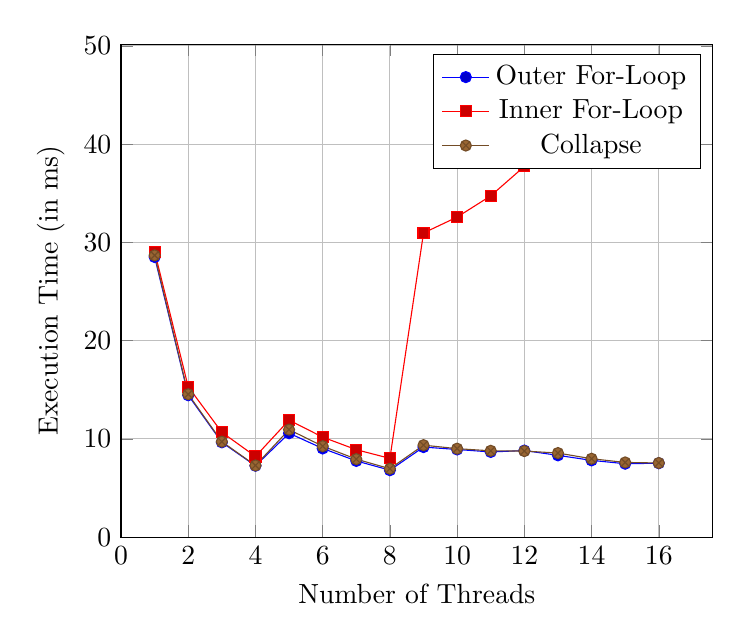
\begin{tikzpicture}
                \begin{axis}[
                    title={},
                    width=0.75\textwidth,
                    xlabel={Number of Threads},
                    ylabel={Execution Time (in ms)},
                    xmin=0,
                    ymin=0,
                    grid=major
                ]
                    \addplot coordinates {
                        (1,28.5091)(2,14.4423)(3,9.64995)(4,7.2662)(5,10.5784)(6,9.026)(7,7.75995)(8,6.8153)(9,9.16705)(10,8.92365)(11,8.67125)(12,8.8138)(13,8.32645)(14,7.8145)(15,7.4751)(16,7.5229)

                    };
                    \addlegendentry{Outer For-Loop}
    
                    \addplot coordinates {
                        (1,29.0502)(2,15.2978)(3,10.6722)(4,8.21485)(5,11.911)(6,10.178)(7,8.9016)(8,8.0159)(9,30.952)(10,32.5705)(11,34.7323)(12,37.7293)(13,38.9948)(14,41.3085)(15,42.0103)(16,45.614)
                    };
                    \addlegendentry{Inner For-Loop}
    
                    \addplot coordinates {
                        (1,28.6757)(2,14.5456)(3,9.71935)(4,7.29605)(5,10.9449)(6,9.2613)(7,7.94005)(8,6.96505)(9,9.3628)(10,9.0075)(11,8.78785)(12,8.76115)(13,8.56025)(14,7.98055)(15,7.60535)(16,7.54825)
                    };
                    \addlegendentry{Collapse}
                \end{axis}
            \end{tikzpicture}
        \caption{Emboss Performance Tests}
        \end{figure}
    \end{center}
\end{frame}
